\documentclass{scrartcl}% ===> this file was generated automatically by noweave --- better not edit it

\usepackage{noweb}
\noweboptions{smallcode,longchunks,longxref}

\usepackage[T1]{fontenc}
%\usepackage{imfellEnglish}
%\usepackage[default]{gillius}
\usepackage{CormorantGaramond}
%\usepackage[el,nf]{coelacanth}
\usepackage[zerostyle=d]{newtxtt}
%\usepackage{FiraMono}

\usepackage[utf8]{inputenc}
% \usepackage[french]{babel}

\usepackage{xcolor}
\definecolor{mygray}{rgb}{0.4,0.4,0.4}
\usepackage[bookmarks,backref=page,linkcolor=mygray]{hyperref} %,colorlinks
\hypersetup{%
  pdfauthor = {Bernard Tatin},
  pdftitle = {},
  pdfsubject = {},
  pdfkeywords = {},
  colorlinks=true,
  linkcolor= mygray,
  citecolor= black,
  pageanchor=true,
  urlcolor = mygray,
  plainpages = false,
  linktocpage
}

\let\oldabstract\abstract
\renewenvironment{abstract}[1]{%
  \hfill
  \begin{minipage}
    {0.95\textwidth}
    \rule{\textwidth}{1pt}
    \footnotesize
    #1
    \normalsize
    {%
      \par\noindent
      \rule{\textwidth}{1pt}
    }
  \end{minipage}
}
%% format des paragraphes
%% \setlength{\parindent}{0cm}
%% \setlength{\parskip}{4mm}
%% \linespread{1.1}
%% \let\nwdocspar=\smallbreak

\newenvironment{packed_itemize}{
\begin{itemize}
  \setlength{\itemsep}{0pt}
  \setlength{\parskip}{0pt}
  \setlength{\parsep}{0pt}
}{\end{itemize}}

%
%
% \usepackage{typearea}
\usepackage{tikz}
\makeatletter
  \setkomafont{section}{\color{white}%
    \bfseries\Large
    \begin{tikzpicture}[overlay]
    \draw[fill=orange] (0,-2pt) rectangle
    (\linewidth,16.4pt);
    \end{tikzpicture}}


\author{Bernard Tatin}
\date{2013/2017}
\title{rbuffer.h, un buffer tournant}
\begin{document}

\pagestyle{noweb}
\maketitle
\abstract{Voici un premier essai de \emph{literate programming}, concept inventé par D. Knuth il y a plus de trente ans. À partir de ce seul fichier on génère la documentation et le code. Ici, je reprend du vieux code, cela m'oblige, même s'il est simple, à le repenser et donc, espérons le, à l'améliorer. Même si je passe beaucoup de temps sur la présentation...}
\tableofcontents
\section{rbuffer}

C'est un buffer tournant le plus simple possible, capable de gérer des lignes délimitées par \emph{LF} (\texttt{'$\backslash$n'}) mais \emph{CR} (\texttt{'$\backslash$r'}) n'est pas pris en compte, plus exactement, il est rejetté.

\subsection{premières définitions}
Pour limiter les calculs, le code..., la taille du buffer est une puissance de 2 d'où la définition du nombre de bits qui ouvre le bal :

\nwfilename{rbuffer.nw}\nwbegincode{1}\sublabel{NWhQHnA-2Sh6y8-1}\nwmargintag{{\nwtagstyle{}\subpageref{NWhQHnA-2Sh6y8-1}}}\moddef{intro-bits~{\nwtagstyle{}\subpageref{NWhQHnA-2Sh6y8-1}}}\endmoddef\nwstartdeflinemarkup\nwusesondefline{\\{NWhQHnA-1p0Y9w-1}}\nwprevnextdefs{\relax}{NWhQHnA-2Sh6y8-2}\nwenddeflinemarkup
#define \nwlinkedidentc{_RBUFFER_BITS}{NWhQHnA-2Sh6y8-1}   8\nwindexdefn{\nwixident{{\_}RBUFFER{\_}BITS}}{:unRBUFFER:unBITS}{NWhQHnA-2Sh6y8-1}
\nwalsodefined{\\{NWhQHnA-2Sh6y8-2}\\{NWhQHnA-2Sh6y8-3}}\nwused{\\{NWhQHnA-1p0Y9w-1}}\nwidentdefs{\\{{\nwixident{{\_}RBUFFER{\_}BITS}}{:unRBUFFER:unBITS}}}\nwendcode{}\nwbegindocs{2}\nwdocspar

La taille du buffer sera donc :

\nwenddocs{}\nwbegincode{3}\sublabel{NWhQHnA-2Sh6y8-2}\nwmargintag{{\nwtagstyle{}\subpageref{NWhQHnA-2Sh6y8-2}}}\moddef{intro-bits~{\nwtagstyle{}\subpageref{NWhQHnA-2Sh6y8-1}}}\plusendmoddef\nwstartdeflinemarkup\nwusesondefline{\\{NWhQHnA-1p0Y9w-1}}\nwprevnextdefs{NWhQHnA-2Sh6y8-1}{NWhQHnA-2Sh6y8-3}\nwenddeflinemarkup
#define \nwlinkedidentc{RBUFFER_SIZE}{NWhQHnA-2Sh6y8-2}    (1 \nwindexdefn{\nwixident{RBUFFER{\_}SIZE}}{RBUFFER:unSIZE}{NWhQHnA-2Sh6y8-2}<< \nwlinkedidentc{_RBUFFER_BITS}{NWhQHnA-2Sh6y8-1})
\nwused{\\{NWhQHnA-1p0Y9w-1}}\nwidentdefs{\\{{\nwixident{RBUFFER{\_}SIZE}}{RBUFFER:unSIZE}}}\nwidentuses{\\{{\nwixident{{\_}RBUFFER{\_}BITS}}{:unRBUFFER:unBITS}}}\nwindexuse{\nwixident{{\_}RBUFFER{\_}BITS}}{:unRBUFFER:unBITS}{NWhQHnA-2Sh6y8-2}\nwendcode{}\nwbegindocs{4}\nwdocspar
Et le masque permettant un rapidide \emph{modulo} arithmétique avec un {\Tt{}and\nwendquote} binaire :
\nwenddocs{}\nwbegincode{5}\sublabel{NWhQHnA-2Sh6y8-3}\nwmargintag{{\nwtagstyle{}\subpageref{NWhQHnA-2Sh6y8-3}}}\moddef{intro-bits~{\nwtagstyle{}\subpageref{NWhQHnA-2Sh6y8-1}}}\plusendmoddef\nwstartdeflinemarkup\nwusesondefline{\\{NWhQHnA-1p0Y9w-1}}\nwprevnextdefs{NWhQHnA-2Sh6y8-2}{\relax}\nwenddeflinemarkup
#define \nwlinkedidentc{RBUFFER_MASK}{NWhQHnA-2Sh6y8-3}    (\nwlinkedidentc{RBUFFER_SIZE}{NWhQHnA-2Sh6y8-2} - 1)\nwindexdefn{\nwixident{RBUFFER{\_}MASK}}{RBUFFER:unMASK}{NWhQHnA-2Sh6y8-3}

\nwused{\\{NWhQHnA-1p0Y9w-1}}\nwidentdefs{\\{{\nwixident{RBUFFER{\_}MASK}}{RBUFFER:unMASK}}}\nwidentuses{\\{{\nwixident{RBUFFER{\_}SIZE}}{RBUFFER:unSIZE}}}\nwindexuse{\nwixident{RBUFFER{\_}SIZE}}{RBUFFER:unSIZE}{NWhQHnA-2Sh6y8-3}\nwendcode{}\nwbegindocs{6}\nwdocspar
\subsection{la structure}

\textbf{\textit{Note: }} tous les membres de la structure sont définis comme {\Tt{}volatile\nwendquote}. C'est important dans un système embarqué avec des interruptions pouvant manipuler le buffer. Sans {\Tt{}volatile\nwendquote}, une optimisation trop agressive pourrait placer une des valeurs entières dans un registre. En cas d'interruption modifiant cette valeur, le registre, lui, ne bougera pas et des caractères pourraient se perdre.

\nwenddocs{}\nwbegincode{7}\sublabel{NWhQHnA-35IAXm-1}\nwmargintag{{\nwtagstyle{}\subpageref{NWhQHnA-35IAXm-1}}}\moddef{tsrbuffer~{\nwtagstyle{}\subpageref{NWhQHnA-35IAXm-1}}}\endmoddef\nwstartdeflinemarkup\nwenddeflinemarkup
/**
 * @struct \nwlinkedidentc{TSrbuffer}{NWhQHnA-35IAXm-1}
 * La structure gérant le buffer tournant.
 */
typedef struct \{
    volatile int in;
    volatile int out;
    volatile int line_count;
    volatile char buffer[\nwlinkedidentc{RBUFFER_SIZE}{NWhQHnA-2Sh6y8-2}];
\} \nwlinkedidentc{TSrbuffer}{NWhQHnA-35IAXm-1};\nwindexdefn{\nwixident{TSrbuffer}}{TSrbuffer}{NWhQHnA-35IAXm-1}

\nwnotused{tsrbuffer}\nwidentdefs{\\{{\nwixident{TSrbuffer}}{TSrbuffer}}}\nwidentuses{\\{{\nwixident{RBUFFER{\_}SIZE}}{RBUFFER:unSIZE}}}\nwindexuse{\nwixident{RBUFFER{\_}SIZE}}{RBUFFER:unSIZE}{NWhQHnA-35IAXm-1}\nwendcode{}\nwbegindocs{8}\nwdocspar
\subsubsection{les champs}
\subsubsection{remarques diverses}
On pourrait définir un {\Tt{}VOLATILE\nwendquote} en fonction de l'architecture du type :

\nwenddocs{}\nwbegincode{9}\sublabel{NWhQHnA-43E2er-1}\nwmargintag{{\nwtagstyle{}\subpageref{NWhQHnA-43E2er-1}}}\moddef{define-volatile~{\nwtagstyle{}\subpageref{NWhQHnA-43E2er-1}}}\endmoddef\nwstartdeflinemarkup\nwusesondefline{\\{NWhQHnA-1p0Y9w-1}}\nwenddeflinemarkup
#if defined(__with_irqs)
  #define VOLATILE volatile
#else
  #define VOLATILE
#endif

\nwused{\\{NWhQHnA-1p0Y9w-1}}\nwendcode{}\nwbegindocs{10}\nwdocspar
Ce qui donnerait au final :

\nwenddocs{}\nwbegincode{11}\sublabel{NWhQHnA-2grPBU-1}\nwmargintag{{\nwtagstyle{}\subpageref{NWhQHnA-2grPBU-1}}}\moddef{tsrbuffer-final~{\nwtagstyle{}\subpageref{NWhQHnA-2grPBU-1}}}\endmoddef\nwstartdeflinemarkup\nwusesondefline{\\{NWhQHnA-1p0Y9w-1}}\nwenddeflinemarkup
/**
 * @struct \nwlinkedidentc{TSrbuffer}{NWhQHnA-35IAXm-1}
 * La structure gérant le buffer tournant.
 */
typedef struct \{
    VOLATILE int in;
    VOLATILE int out;
    VOLATILE int line_count;
    VOLATILE char buffer[\nwlinkedidentc{RBUFFER_SIZE}{NWhQHnA-2Sh6y8-2}];
\} \nwlinkedidentc{TSrbuffer}{NWhQHnA-35IAXm-1};\nwindexdefn{\nwixident{TSrbuffer}}{TSrbuffer}{NWhQHnA-2grPBU-1}
\nwindexdefn{\nwixident{TSrbuffer}}{TSrbuffer}{NWhQHnA-2grPBU-1}\eatline
\nwused{\\{NWhQHnA-1p0Y9w-1}}\nwidentdefs{\\{{\nwixident{TSrbuffer}}{TSrbuffer}}}\nwidentuses{\\{{\nwixident{RBUFFER{\_}SIZE}}{RBUFFER:unSIZE}}}\nwindexuse{\nwixident{RBUFFER{\_}SIZE}}{RBUFFER:unSIZE}{NWhQHnA-2grPBU-1}\nwendcode{}\nwbegindocs{12}\nwdocspar
\nwenddocs{}\nwbegindocs{13}\nwdocspar

\subsection{le fonctionnement}
\subsubsection{ajout d'un caractère}
Le fonctionnement est le suivant pour l'ajout d'un caractère :

\begin{packed_itemize}
  \item si le caractère est '$\backslash$r', on ne fait rien,
  \item on place le caractère dans le buffer à la position {\Tt{}in\nwendquote},
  \item on incrémente {\Tt{}in\nwendquote},
  \item si on atteint la limite du buffer, on positionne {\Tt{}in\nwendquote} à 0,
  \item si le caractère est '$\backslash$n', on incrémente {\Tt{}line{\_}count\nwendquote}.
\end{packed_itemize}

\nwenddocs{}\nwbegincode{14}\sublabel{NWhQHnA-4LzvSl-1}\nwmargintag{{\nwtagstyle{}\subpageref{NWhQHnA-4LzvSl-1}}}\moddef{add-char~{\nwtagstyle{}\subpageref{NWhQHnA-4LzvSl-1}}}\endmoddef\nwstartdeflinemarkup\nwusesondefline{\\{NWhQHnA-1p0Y9w-1}}\nwenddeflinemarkup
static INLINE void \nwlinkedidentc{rbf_add_char}{NWhQHnA-4LzvSl-1}(\nwlinkedidentc{TSrbuffer}{NWhQHnA-35IAXm-1} *rb, const char c) \{\nwindexdefn{\nwixident{rbf{\_}add{\_}char}}{rbf:unadd:unchar}{NWhQHnA-4LzvSl-1}
    if (c != '\\r') \{
        rb->buffer[rb->in++] = c;
        rb->in &= \nwlinkedidentc{RBUFFER_MASK}{NWhQHnA-2Sh6y8-3};
        if (c == '\\n') \{
            rb->line_count++;
        \}
    \}
\}


\nwused{\\{NWhQHnA-1p0Y9w-1}}\nwidentdefs{\\{{\nwixident{rbf{\_}add{\_}char}}{rbf:unadd:unchar}}}\nwidentuses{\\{{\nwixident{RBUFFER{\_}MASK}}{RBUFFER:unMASK}}\\{{\nwixident{TSrbuffer}}{TSrbuffer}}}\nwindexuse{\nwixident{RBUFFER{\_}MASK}}{RBUFFER:unMASK}{NWhQHnA-4LzvSl-1}\nwindexuse{\nwixident{TSrbuffer}}{TSrbuffer}{NWhQHnA-4LzvSl-1}\nwendcode{}\nwbegindocs{15}\nwdocspar
\subsection{le code final}

\nwenddocs{}\nwbegincode{16}\sublabel{NWhQHnA-1p0Y9w-1}\nwmargintag{{\nwtagstyle{}\subpageref{NWhQHnA-1p0Y9w-1}}}\moddef{*~{\nwtagstyle{}\subpageref{NWhQHnA-1p0Y9w-1}}}\endmoddef\nwstartdeflinemarkup\nwenddeflinemarkup
\LA{}intro-bits~{\nwtagstyle{}\subpageref{NWhQHnA-2Sh6y8-1}}\RA{}
\LA{}define-volatile~{\nwtagstyle{}\subpageref{NWhQHnA-43E2er-1}}\RA{}
\LA{}tsrbuffer-final~{\nwtagstyle{}\subpageref{NWhQHnA-2grPBU-1}}\RA{}
\LA{}add-char~{\nwtagstyle{}\subpageref{NWhQHnA-4LzvSl-1}}\RA{}
\nwnotused{*}\nwendcode{}\nwbegindocs{17}\nwdocspar
\section{annexes}

\subsection{la ligne de commande}
Pour obtenir le fichier \LaTeX{} et le code source, voici ce qu'il faut faire depuis un terminal :

\nwenddocs{}\nwbegincode{18}\sublabel{NWhQHnA-2CUXU7-1}\nwmargintag{{\nwtagstyle{}\subpageref{NWhQHnA-2CUXU7-1}}}\moddef{command-line~{\nwtagstyle{}\subpageref{NWhQHnA-2CUXU7-1}}}\endmoddef\nwstartdeflinemarkup\nwenddeflinemarkup
# fichier LaTeX
noweave -delay -autodefs c -index rbuffer.nw > rbuffer.tex
# fichier PDF
pdflatex rbuffer.tex && \\
  pdflatex rbuffer.tex && \\
  pdflatex rbuffer.tex
# le code source
notangle rbuffer.nw > rbuffer.h
\nwnotused{command-line}\nwendcode{}

\nwixlogsorted{c}{{*}{NWhQHnA-1p0Y9w-1}{\nwixd{NWhQHnA-1p0Y9w-1}}}%
\nwixlogsorted{c}{{add-char}{NWhQHnA-4LzvSl-1}{\nwixd{NWhQHnA-4LzvSl-1}\nwixu{NWhQHnA-1p0Y9w-1}}}%
\nwixlogsorted{c}{{command-line}{NWhQHnA-2CUXU7-1}{\nwixd{NWhQHnA-2CUXU7-1}}}%
\nwixlogsorted{c}{{define-volatile}{NWhQHnA-43E2er-1}{\nwixd{NWhQHnA-43E2er-1}\nwixu{NWhQHnA-1p0Y9w-1}}}%
\nwixlogsorted{c}{{intro-bits}{NWhQHnA-2Sh6y8-1}{\nwixd{NWhQHnA-2Sh6y8-1}\nwixd{NWhQHnA-2Sh6y8-2}\nwixd{NWhQHnA-2Sh6y8-3}\nwixu{NWhQHnA-1p0Y9w-1}}}%
\nwixlogsorted{c}{{tsrbuffer}{NWhQHnA-35IAXm-1}{\nwixd{NWhQHnA-35IAXm-1}}}%
\nwixlogsorted{c}{{tsrbuffer-final}{NWhQHnA-2grPBU-1}{\nwixd{NWhQHnA-2grPBU-1}\nwixu{NWhQHnA-1p0Y9w-1}}}%
\nwixlogsorted{i}{{\nwixident{{\_}RBUFFER{\_}BITS}}{:unRBUFFER:unBITS}}%
\nwixlogsorted{i}{{\nwixident{rbf{\_}add{\_}char}}{rbf:unadd:unchar}}%
\nwixlogsorted{i}{{\nwixident{RBUFFER{\_}MASK}}{RBUFFER:unMASK}}%
\nwixlogsorted{i}{{\nwixident{RBUFFER{\_}SIZE}}{RBUFFER:unSIZE}}%
\nwixlogsorted{i}{{\nwixident{TSrbuffer}}{TSrbuffer}}%
\nwbegindocs{19}\nwdocspar
L'option {\Tt{}-autodefs\ c\nwendquote} permet à {\Tt{}noweave\nwendquote} de déterminer lui-même les éléments du langage C. Sans cette option, dans le cadre de ce fichier, les définitions de {\Tt{}intro-bits\nwendquote} ne seraient pas visibles.

\section{tables et index}
\subsection{table des extraits de code}

\nowebchunks

\subsection{index}

\nowebindex

\end{document}
\nwenddocs{}
